%%%%%%%%%%%%%%%%%%%%%%%%%%%%%%%%%%%%%%%%%%%%%%%%%%%%%%%%%%%%%%%%%%%%%%%%%%%%%%
%%%%%%%%%%%%%%%%%%%%%%%%%%%%%%%%%%%%%%%%%%%%%%%%%%%%%%%%%%%%%%%%%%%%%%%%%%%%%%
%%
%% Ukázkový příklad dokumentace úkolu do předmětů IZP a IUS, 2010
%%
%% Upravená původní dokumentace od Davida Martinka.
%%%%%%%%%%%%%%%%%%%%%%%%%%%%%%%%%%%%%%%%%%%%%%%%%%%%%%%%%%%%%%%%%%%%%%%%%%%%%%
%%%%%%%%%%%%%%%%%%%%%%%%%%%%%%%%%%%%%%%%%%%%%%%%%%%%%%%%%%%%%%%%%%%%%%%%%%%%%%
\documentclass[12pt,a4paper,titlepage,final]{article}


% cestina a fonty
\usepackage[czech]{babel}
\usepackage[utf8]{inputenc}
% balicky pro odkazy
\usepackage[bookmarksopen,colorlinks,plainpages=false,urlcolor=blue,unicode]{hyperref}
\usepackage{url}
% obrazky
\usepackage[dvipdf]{graphicx}
% velikost stranky
\usepackage[top=3.5cm, left=2.5cm, text={17cm, 24cm}, ignorefoot]{geometry}
\begin{document}

%%%%%%%%%%%%%%%%%%%%%%%%%%%%%%%%%%%%%%%%%%%%%%%%%%%%%%%%%%%%%%%%%%%%%%%%%%%%%%
% titulní strana

% !!!!!!!!!!!!!!!!!!!!!!!!!!!!!!!!!!!!!!!!!!!!!!!!!
% změň následující údaje za své
\def\author{xxx}
\def\email{xxx@stud.fit.vutbr.cz}
\def\projname{Implementace interpretu imperativního jazyka IFJ12}
% !!!!!!!!!!!!!!!!!!!!!!!!!!!!!!!!!!!!!!!!!!!!!!!!!

\begin{titlepage}

% \vspace*{1cm}
\begin{figure}[!h]
  \centering
  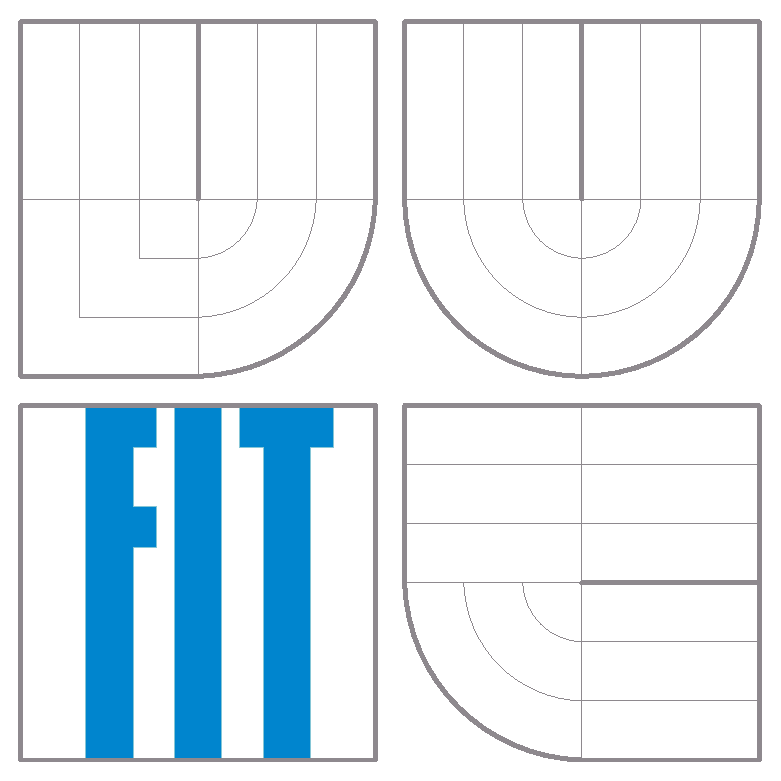
\includegraphics[height=5cm]{img/logo.eps}
\end{figure}

\vfill

\begin{center}
\begin{Large}
Dokumentace k projektu pro předměty IFJ a IAL\\
\end{Large}
\bigskip
\begin{Huge}
\projname\\
\end{Huge}
\begin{large}
Tým 113, varianta a/1/I\\
\end{large}
\textit{Vedoucí týmu: Antonín Marko}\\
\end{center}

\vfill

\begin{center}
\begin{Large}
\today
\end{Large}
\end{center}

\vfill

\begin{flushleft}
%\begin{large}
\begin{tabular}{l l l l l}
\textbf{Řešitelé}: 
&3BIT& Antonín Marko 20\% &\url{xmarko07@stud.fit.vutbr.cz} \\
&1BIT& Tomáš Pružina 20\% &\url{xpruzi01@stud.fit.vutbr.cz} \\
&3BIT& Martin Kubíček 20\% &\url{xkubic34@stud.fit.vutbr.cz} \\
&3BIT& Martin Juřík 20\% &\url{xjurik08@stud.fit.vutbr.cz} \\
&3BIT& Petr David 20\%s &\url{xdavid15@stud.fit.vutbr.cz} \\

%Autor: & \author, \url{\email}  \\
% & Fakulta Informačních Technologií \\
% & Vysoké Učení Technické v~Brně \\
\end{tabular}
\newline
\newline
\textbf{Rozšíření}: ARRAY, REPEAT, ELSEIF, BOOLOP, FOR
%\end{large}
\vfill
\begin{large}
Fakulta Informačních Technologií \\
Vysoké Učení Technické v~Brně \\
\end{large}
\end{flushleft}
\end{titlepage}

%%%%%%%%%%%%%%%%%%%%%%%%%%%%%%%%%%%%%%%%%%%%%%%%%%%%%%%%%%%%%%%%%%%%%%%%%%%%%%
% obsah
\pagestyle{plain}
\pagenumbering{roman}
\setcounter{page}{1}
\tableofcontents

%%%%%%%%%%%%%%%%%%%%%%%%%%%%%%%%%%%%%%%%%%%%%%%%%%%%%%%%%%%%%%%%%%%%%%%%%%%%%%
% textova zprava
\newpage
\pagestyle{plain}
\pagenumbering{arabic}
\setcounter{page}{1}

%%%%%%%%%%%%%%%%%%%%%%%%%%%%%%%%%%%%%%%%%%%%%%%%%%%%%%%%%%%%%%%%%%%%%%%%%%%%%%
\section{Úvod} \label{uvod}
%=============================================================================
Implementacia prekladace imperativneho jazyka je netrivialna uloha, preto je
vhodne ju rozdelit na podulohy (kapitola 2), ktore su vhodne rozdelene medzi
cleny timu, vedeneho a kontrolovaneho timovym veducim.

Tento dokument sa sklada z N casti, ktore popisuju jednotlive moduly
interpretu imperativneho jazyka IFJ14, jakozto lexikalny analyzator (ref),
syntakticky analyzator (ref) vyuzivajuceho rekurzivny sestup (ref), ktory je
pre potreby syntaxtickej analyzy vyrazov rozsireny o Shunting Yard (ref)
algoritmus.
Yadi yadi yada...

%%%%%%%%%%%%%%%%%%%%%%%%%%%%%%%%%%%%%%%%%%%%%%%%%%%%%%%%%%%%%%%%%%%%%%%%%%%%%%
\section{Moduly interpretu jazyka} \label{moduly_interpretu}
%=============================================================================
\subsection{Lexikální analyzátor} \label{lexikalni_analyzator}

Syntakticky analyzator potrebuje ke sve cinnosti lexikalny analyzator. Ten
predava na ziadost SA tzv. takeny, ktore ziskava postupnym citanim vstupneho
suboru, ktory obsahuje zdrojovy kod napisany v jazyku IFJ14.
Samotny vysledny token je reprezentaciou lexemu (identifikator, klicove slovo,
prikaz priradenia atp.).

Pre uspesne rozlisenie typu lexemu sa v nasej implementacii pouziva konecny
automat, ktoreho struktura je znazornena obrazkom (ref).

Ak sa konecny automat pocas spracovavania retazca zdrojoveho suboru dostane do
chyboveho stavu (LEX_ERR (ref)), retazec je neprijaty a jedna sa o lexikalnu
chybu. Samotna implementacia lexikalneho analyzatoru patri k jednoduchsim
castiam projektu, avsak jeho navrh a testovanie zabral nemalo casu (liez).

<insert KA diagram here>


\subsection{Syntaktický analyzátor} \label{syntakticky_analyzator}
\subsubsection{Precedenční syntaktický analyzátor} \label{precedencni_syntakticky_analyzator}
\subsection{Interpret} \label{interpret}

Interpret je zaverecnou castou projektu. Rekurzivne spracovava abstraktny
syntakticky strom reprezentovanym binarnym strom a postupne vykonava operacie
na nom definovane.

Korenom tohto AST je vzdy typ prevadanej operace, pricom obsahuje predom
definovane nepovinne parametre (prikladom je podstrom volania funkcie, ktory
obsahuje predavane premenne). Teda kazdy uzol AST predstavuje jednu atomicku
operaciu, ktorou je riadeny samotny beh programu.

Interpret samozrejme nepracuje len so samotnym syntaktickym stromom, ale
taktiez s tabulkou symbolou, ktora obsahuje data potrebne na to, aby interpret
mohol vykonavat nejaku uzitocnu praca definovanu v tele programu.

Interpret teda spravuje tabulky symbolov, dynamicky ich za behu
vykonavaneho programu vytvara a (podla potreby) rusi.

V neposlednej rade interpret vykonava semanticku kotrolu pri operaciach, ktore
nie je syntakticky analyzator v dobe spracovanaia vstupneho programu a generacie
abstraktneho syntaktickeho stromu riesit.

Prikladom takejto kontroly je pouzivanie (citanie) premennej pred jej riadnou
definicou (priradenim hodnoty) alebo delenie nulou v aritmetickom vyraze.

Taketo behove chyby su v interprete riesene ukoncenim interpretacia a navratom
chyboveho kodu podla zadania imperativneho jazyka IFJ14.

\subsubsection{Tabulka symbolů} \label{tabulka_symbolu}

Tabulka symbolov je implementovana pomocou binarnecho vyhladavacieho stromu,
pricom sa rozlisuje niekolko urovni tabulky symbolov.

Kazdy program obsahuje globalnu tabulku symbolov (v ktorej su ulozene ukazatele
na funkcie) a lokalnu tabulku symbolov, ktora obsahuje behove premenne
vykonavaneho programu.

Interpret spravuje tabulk

Z implentacneho hladiska su lokalne tabulky symbolov (stromy) ukladane na
zasobnik, pricom plati, ze pri volani funkcie sa vytvori nova (lokalna)
tabulka symbolov, do ktorej sa skopiruju prislusne parametre volanej funkcie z
nizsej vrstvy lokalnej tabulky (popr. z globalnej tabulky symbolov).

Takato lokalna tabulky taktiez obsahuje navratovu hodnotu vykonavanej funkcie,
co umoznuje rekurzivne volanie funkcii a samozrejme umoznuje vykonavat telo
funkcie bez nutnosti akokolvek zasahovat do abstraktneho syntaktickeho stromu.


%%%%%%%%%%%%%%%%%%%%%%%%%%%%%%%%%%%%%%%%%%%%%%%%%%%%%%%%%%%%%%%%%%%%%%%%%%%%%%
\section{Postup při implementaci řešení} \label{postup_pri_implementaci_reseni}
%=============================================================================

%%%%%%%%%%%%%%%%%%%%%%%%%%%%%%%%%%%%%%%%%%%%%%%%%%%%%%%%%%%%%%%%%%%%%%%%%%%%%%
\section{Závěr} \label{zaver}
%%%%%%%%%%%%%%%%%%%%%%%%%%%%%%%%%%%%%%%%%%%%%%%%%%%%%%%%%%%%%%%%%%%%%%%%%%%%%

\appendix

\section{Metriky kódu} \label{metriky}

%%%%%%%%%%%%%%%%%%%%%%%%%%%%%%%%%%%%%%%%%%%%%%%%%%%%%%%%%%%%%%%%%%%%%%%%%%%%%%
% seznam citované literatury: každá položka je definována příkazem
% \bibitem{xyz}, kde xyz je identifikátor citace (v textu použij: \cite{xyz})
\begin{thebibliography}{1}

% jedna citace:
\bibitem{honzik}
HONZÍK J. M.: \emph{Studijní opora pro předmět Algoritmy}. Elektronický text. FIT VUT v Brně
\bibitem{meduna}
MEDUNA A., LUKÁŠ R., \emph{Podklady k přednáškám}. Elektronický text. FIT VUT v Brně


\end{thebibliography}
%%%%%%%%%%%%%%%%%%%%%%%%%%%%%%%%%%%%%%%%%%%%%%%%%%%%%%%%%%%%%%%%%%%%%%%%%%%%%%
\appendix

\end{document}

